%
% chapter.tex -- Kapitel 2: Koordinaten und Tangentialvektoren
%
% (c) 2024 Prof Dr Andreas Müller
%
\chapter{Koordinaten und Tangentialvektoren
\label{chapter:koordinaten}}
\kopflinks{Koordinaten und Tangentialvektoren}
Die Bühne der Physik ist ein Raum von Punkten, in dem wir geometrische
Konstruktionen anwenden und zum Beispiel Bahnen von Körpern beschreiben
können.
Solche Beschreibungen verwenden immer mehr oder weniger speziell gewählte
Koordinatensysteme, die Punkte durch Koordinaten beschreiben.
Da die Koordinaten nur ein Werkzeug zur physikalischer Gegebenheiten
sind, muss es immer möglich sein, die zur Formulierung von Naturgesetzen
entwickelten Abstraktionen wie Kurven, Funktionen oder Vektoren zwischen
beliebigen Koordinatensystemen umzurechnen.
Ziel dieses Kapitels ist daher, eine für alle Arten von Koordinatensystemen
nützliche Notation zu entwickeln, die Umrechnung zwischen Koordinatensystemen
zu studieren und den Begriff des Tangentialvektors einzuführen.

%
% Koordinaten
%
\section{Koordinaten
\label{buch:koordinaten:section:koordinaten}}
\kopfrechts{Koordinaten}
In diesem Abschnitt betrachten wir eine Punktmenge $X$, die mit
Koordinatensystemen ausgestattet werden soll.
Ohne das Koordinatensystem hat die Punktemenge keinerlei Struktur.
Um von stetigen Abbildungen zwischen solchen Mengen zu sprechen,
wird zum Beispiel ein Begriff der Nähe benötigt, mit dem die Konvergenz
von Folgen definiert werden kann.
Die Konstruktion eines Koordinatensystems ermöglicht, Punkte also
nahe beeinander zu betrachten, wenn sich ihre Koordinaten nur geringfügig
unterscheiden.

\subsection{Koordinatensystem}
%
% fig-koordinaten.tex
%
% (c) 2024 Prof Dr Andreas Müller
%
\begin{figure}
\centering
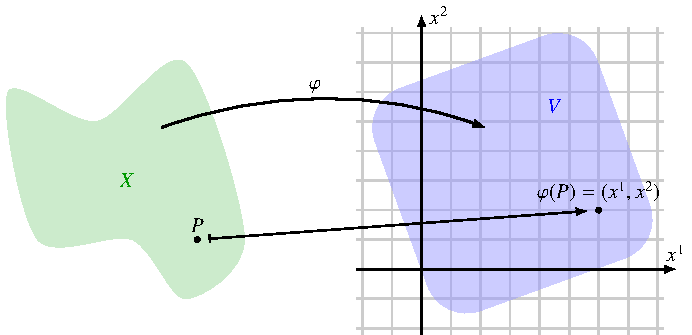
\includegraphics{chapters/020-koordinaten/images/koordinaten.pdf}
\caption{Ein Koordinatensystem auf der Punktmenge $X$ ist eine Abbildung 
$\varphi$ in den Koordinatenraum $V$, der eine Teilmenge von
$\mathbb{R}^n$ ist.
\label{buch:koordinaten:koordinaten:fig:koordinaten}}
\end{figure}
%
Ein $n$-dimensionales Koordinatensystem auf $X$ ordnet jedem Punkt 
ein $n$-Tupel von Koordinaten zu.
Aus erst später verständlichen Gründen bezeichnen wir die Koordinaten
mit hochgestellten Indizes, wir schreiben also $x^1,\dots,x^n$.
Eine Verwechslungsgefahr mit Exponenten besteht normalerweise nicht.
Falls die $k$-te Potenz der Koordinate $x^1$ berechnet werden soll, 
wird dies mit Klammern als $(x^i)^k$ geschrieben.
Ein Koordinatensystem ist also eine Abbildung
\[
\varphi
\colon
X\to \mathbb{R}^n
:
P \mapsto (x^1,\dots,x^n),
\]
wie sie in Abbildung~\ref{buch:koordinaten:koordinaten:fig:koordinaten}
dargestellt ist.
Jede einzelne Koordinate kann als Funktion $P\mapsto x^i(P)$ mit
reellen Werten betrachtet werden.

\begin{beispiel}
\label{buch:koordinaten:koordinaten:beispiel:kartpolar}
%
% fit-kartpolar.tex%
%
% (c) 2024 Prof Dr Andreas Müller
%
\begin{figure}
\centering
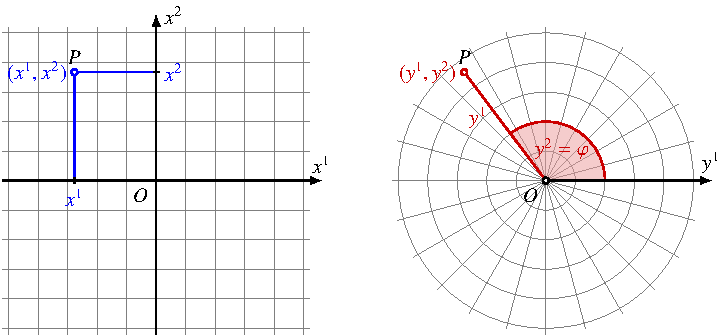
\includegraphics{chapters/020-koordinaten/images/kartpolar.pdf}
\caption{Zwei Koordinatensysteme für die Ebene:
kartesische (rechtwinklige) Koordinaten links und Polarkoordinaten
rechts.
Der gleiche Punkt $P$ wird gleichermassen durch die Koordinaten 
$(x^1,x^2)$ und $(y^1,y^2)$ beschrieben.
\label{buch:koordinaten:fig:kartpolar}}
\end{figure}

Die Punkte einer Ebene können einerseits mit dem {\em kartesischen}
Koordinatensystem mit den Koordinaten $(x^1,x^2)\in\mathbb{R}$ 
beschrieben werden und andererseits durch {\em Polarkoordinaten},
\index{Polarkoordinaten}%
die einen Punkt durch den Radius $y^1 = r$ und den Polarwinkel
$y^2 = \varphi$ definieren (Abbildung~\ref{buch:koordinaten:fig:kartpolar}).

Die kartesischen Koordinaten können aus den Polarkoordinaten durch
\begin{equation}
\left.
\begin{aligned}
x^1 &= y^1\cos y^2 \\
x^2 &= y^1\sin y^2
\end{aligned}
\qquad
\right\}
\label{buch:koordinaten:koordinaten:eqn:polarkartumrechnung}
\end{equation}
berechnet werden.
\end{beispiel}

\begin{beispiel}
\label{buch:koordinaten:koordinaten:beispiel:kartkugel}
%
% fig-kartkugel.tex
%
% (c) 2024 Prof Dr Andreas Müller
%
\begin{figure}
\centering
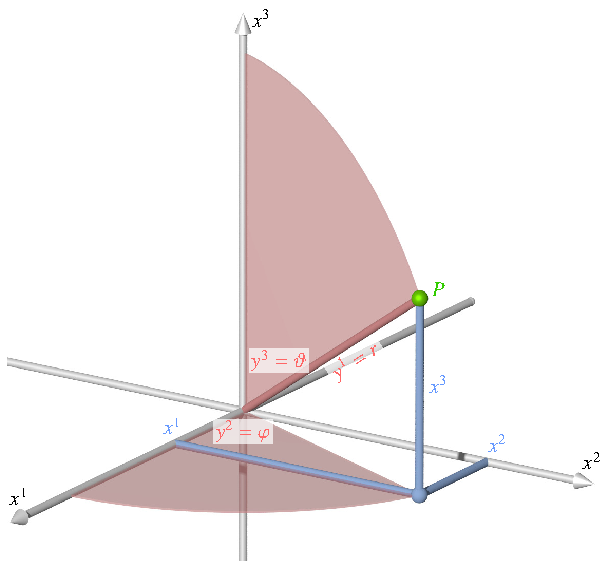
\includegraphics{chapters/020-koordinaten/images/kartkugel.pdf}
\caption{Kartesische Koordinaten ({\color{blue}blau}) und Kugelkoordinaten
({\color{darkred}rot}) für einen Punkt $P$ des dreidmensionalen Raumes.
\label{buch:koordinaten:koordinaten:fig:kartkugel}}
\end{figure}

Der dreidimensionale Raum kann sowohl durch {\em kartesische}
Koordinatentripel $(x^1,x^2,x^3)$ wie auch durch {\em Kugelkoordinaten}
\index{Kugelkoordinaten}%
beschrieben werden.
In Kugelkoordinaten ist ein Punkt durch die Entfernung $r=y^1$ vom
Nullpunkt, den Polarwinkel $y^2=\varphi$ seiner Projektion in die 
$x^1$-$x^2$-Ebene und den Winkel $\vartheta$ zwischen der positiven
$x^3$-Achse und der Geraden durch Nullpunkt $O$ und den Punkt gegeben
(Abbildung~\ref{buch:koordinaten:koordinaten:fig:kartkugel}).
Die Umrechnung von Kugelkoordinaten in kartesische Koordinaten
erfolgt mit
\begin{equation}
\left.
\begin{aligned}
x^1
&=
y^1 \cos y^2 \cos y^3 \\
x^2
&=
y^1 \sin y^2 \cos y^3 \\
x^3
&=
y^2 \cos y^3.
\end{aligned}
\qquad\right\}
\label{buch:koordinaten:koordinaten:eqn:kugelkartumrechnung}
\end{equation}
Man beachte, dass Punkte auf der $x^3$-Achse $y^3=0$ oder
$y^3=\pi$ und beliebigen Winkel $y^2\in\mathbb{R}$ haben.
Ohne zusätzliche Einschränkungen haben die Punkte auf der
$x^3$-Achse keine eindeutigen Kugelkoordinaten.
\end{beispiel}


Um die Struktur des Koordinatenraumes $\mathbb{R}^n$ auf die Menge
$X$ zu übertragen, müssen die Koordinatenabbildungen weiter eingeschränkt
werden.
Zunächst muss die Koordinatenabbildung bijektiv sein.
Dies bedeutet, dass jeder Punkt durch genau ein Koordinaten-$n$-Tupel
beschrieben wird.
Diese Bedingung ist in beiden Beispielen nicht erfüllt, da Tupel,
deren $y^2=\varphi$-Koordinaten sich um $2\pi$ unterscheiden, den
gleichen Punkt beschreiben.
Sie ist aber für genügend kleine Teilmengen des Raumes erfüllt.

Tatsächlich kann man nicht erwarten, zum Beispiel die Oberfläche einer
Kugel oder eines Torus in ihrer Gesamtheit eineindeutig auf Ebene
abzubilden.
Die Definition eines Koordinatensystems ist vorerst also nur geeignet,
eine Punktmenge lokal zu beschreiben.
Für eine globale Beschreibung wird es notwendig sein, verschiedene
Koordinatensysteme, die auf Teilen einer Menge definiert sind, zu
einem grösseren Ganzen zusammenzufügen.

Ausserdem muss die Menge $V=\varphi(X)$ der möglichen Koordinaten-$n$-Tupel
eine offene Menge in $\mathbb{R}^n$ sein.
Auch diese Bedingung ist in den Beispielen nicht erfüllt.
Die $y^1=r$-Koordinate nimmt alle Werte in
\[
\mathbb{R}_{\ge 0}
=
[0,\infty)
=
\{
y^1\in\mathbb{R}
\mid
y^1\ge 0
\}.
\]
Dies ist keine offene Menge, da die Punkte $(0,y^2)$ bzw.~$(0,y^2,y^3)$
ein Randpunkt des Wertebereichs der $y$-Koordinaten ist.
Bei Kugelkoordinaten nimmt die Koordinate $y^3$ Werte im
abgeschlossenen Interval $[0,\pi]$ an, was zu weiteren Randpunkten
des Wertebereichs führen.

% XXX Beispiel zur Notwendigkeit der letzten Bedingung zeigen

\subsection{Koordinatenwechsel}
In den Beispielen
\ref{buch:koordinaten:koordinaten:beispiel:kartpolar}
und
\ref{buch:koordinaten:koordinaten:beispiel:kartkugel}
wurden bereits Umrechnungsformeln zwischen den dort dargestellten
Koordinatensystemen ermittelt.
Seien etwas allgemeiner zwei Koordinatensysteme $x^1,\dots,x^n$
und $y^1,\dots,y^n$ auf der Punktmenge $X$ gegeben.
Wenn $U$ die Menge der Koordinaten-$n$-Tupel ist, die Punkte von $X$
in den $x^i$-Koordinaten beschreiben, dann ist die Koordinatenumrechnung
vom $x^i$-Koordinatensystem in das $y^i$-Koordinatensystem eine Abbildung
\[
\varphi
\colon
U\to\mathbb{R}^n
:
(x^1,\dots,x^n)
\mapsto
(y^1,\dots,y^n)
\]
von $U$ in $\mathbb{R}^n$.


\subsubsection{Stetigkeit}

\subsubsection{Differenzierbarkeit}

\subsubsection{Topologische Räume}

%
% Tangentialvektoren
%
\section{Tangentialvektoren
\label{buch:koordinaten:section:tangentialvektoren}}
\kopfrechts{Tangentialvektoren}

%
% Differentialoperatoren
%
\section{Differentialoperatoren
\label{buch:koordinaten:section:differentialoperatoren}}
\kopfrechts{Differentialoperatoren}

%
% Differenzierbare Atlanten und differenzierbare Mannigkfaltigkeiten
%
\section{Differenzierbare Mannigfaltigkeiten
\label{buch:koordinatne:section:mannigfaltigkeiten}}
\kopfrechts{Differenzierbare Mannigfaltigkeiten}



